\documentclass{article}
\usepackage[utf8]{inputenc}
\usepackage{graphicx}

\usepackage{amsthm, amsmath, amssymb, amsfonts, epsfig}
\usepackage{algorithm, algpseudocode}
\usepackage{algcompatible}
%%%%%%%%%%%%%%%%% this version: 03-14-2017 %%%%%%%%%%%%%%%%%%%%%%%%%%%%%%%

%%% standard packages
\usepackage{amsthm, amsmath, amssymb, amsfonts, graphicx, epsfig}
%\graphicspath{ {D:/Notes/others/assets/} }

\usepackage{algorithm, algpseudocode}

\allowdisplaybreaks
\usepackage{setspace}
%\usepackage{accents}
%%%
%\usepackage{kbordermatrix}

%%%%%%%%%%%%%%%%%%%%%%% ADDITIONAL FONTS %%%%%%%%%%%%%%%%%%%%%%%%%%%%%%
%%% Package to make \mathbbm, in particular to have 1 as for indicator function
\usepackage{bbm}
%%% Package to make special curl fonts, by using \mathscr{F}
\usepackage{mathrsfs}
%%% dsfont sometimes used instead of mathbb or mathbbm
%\usepackage{dsfont}
%%%%%%%%%%%%%%%%%%%%%%%%%%%%%%%%%%%%%%%%%%%%%%%%%%%%%%%%%%%%%%%%%%%%%%%


%%%%%%%%%%%%%%%%%%%%%%%%%%%%%%%%%%%%%%%%%%%%%%%%%%%%%%%%%%%%%%%%%%%%%%
%%% The ulem package provides various types of underlining that can
%%% stretch between words and be broken across lines. Convenient for editing. \sout{xxxx}
%%% http://ctan.unixbrain.com/macros/latex/contrib/ulem/ulem.pdf
%%%% Remark: if used with natbib, then the bibliography comes underlined. Comment this package at last compilation
%\usepackage{ulem}
%%%%%%%%%%%%%%%%%%%%%%%%%%%%%%%%%%%%%%%%%%%%%%%%%%%%%%%%%%%%%%%%%%%%%%

%%%%%%%%%%%%%%%%%%%%%%%%%%%%%%%%%%%%%%%%%%%%%%%%%%%%%%%%%%%%%%%%%%%%%%
%% Cancel is used to cross out in math mode. \xcancel, \cancel Convenient for editting.
%% http://ctan.math.utah.edu/ctan/tex-archive/macros/latex/contrib/cancel/cancel.pdf
%\usepackage{cancel}
%%%%%%%%%%%%%%%%%%%%%%%%%%%%%%%%%%%%%%%%%%%%%%%%%%%%%%%%%%%%%%%%%%%%%%


%%%%%%%%%%%%%%%%%%%%%%%%%%%%%%%%%%%%%%%%%%%%%%%%%%%%%%%%%%%%%%%%%%%%%%%
%This packages adds support of handling eps images to package graphics
%or graphicx with option pdftex. If an eps image is detected, epstopdf is
%automatically called to convert it to pdf format.
\usepackage{epstopdf}
%%%%%%%%%%%%%%%%%%%%%%%%%%%%%%%%%%%%%%%%%%%%%%%%%%%%%%%%%%%%%%%%%%%%%%%


%%%%%%%%%%%%%%%%%%%%%%%%%%%%%%%%%%%%%%%%%%%%%%%%%%%%%%%%%%%%%%%%%%%%%%%
% various features for using graphics, including subfigure, captions, subcaptions etc.
\usepackage{graphicx}
%\usepackage{caption}
\usepackage[font=sl,labelfont=bf]{caption}
\usepackage{subcaption}
%%%%%%%%%%%%%%%%%%%%%%%%%%%%%%%%%%%%%%%%%%%%%%%%%%%%%%%%%%%%%%%%%%%%%%%


%%%%%%%%%%%%%%%%%%%%%%%%%%%%%%%%%%%%%%%%%%%%%%%%%%%%%%%%%%%%%%%%%%%%%%%
% This package improves the interface for defining floating objects such
% as figures and tables in LaTeX.
% http://www.ctan.org/pkg/float
\usepackage{float}
\restylefloat{table}
%%%%%%%%%%%%%%%%%%%%%%%%%%%%%%%%%%%%%%%%%%%%%%%%%%%%%%%%%%%%%%%%%%%%%%%


%%% use for diagonals in the table's cells
%\usepackage{slashbox}  %Removed by Ares

%%%%%%%%%%%%%%%%%%%%%%%%%%%%%%%%%%%%%%%%%%%%%%%%%%%%%%%%%%%%%%%%%%%%%%%


%%%%%%%%%%%%%%%%%%%%%%%%%%%%%%%%%%%%%%%%%%%%%%%%%%%%%%%%%%%%%%%%%%%%%%%
% This package gives the enumerate environment an optional argument
% which determines the style in which the counter is printed.
% http://www.ctex.org/documents/packages/table/enumerate.pdf
\usepackage{enumerate}
%%%%%%%%%%%%%%%%%%%%%%%%%%%%%%%%%%%%%%%%%%%%%%%%%%%%%%%%%%%%%%%%%%%%%%%


%%%%%%%%%%%%%%%%%%%%%%%%%%%%%%%%%%%%%%%%%%%%%%%%%%%%%%%%%%%%%%%%%%%%%%%
%selectively in/exclude pieces of text: the user can determine new comment versions,
%and each is controlled separately. Special comments can be determined where the
%user specifies the action that is to be taken with each comment line.
% http://get-software.net/macros/latex/contrib/comment/comment.pdf
%\usepackage{comment}
%%%%%%%%%%%%%%%%%%%%%%%%%%%%%%%%%%%%%%%%%%%%%%%%%%%%%%%%%%%%%%%%%%%%%%%


%%%%%%%%%%%%%%%%%%%%%%%%%%%%%%%%%%%%%%%%%%%%%%%%%%%%%%%%%%%%%%%%%%%%%%
%% To display the labels used in a tex file in the dvi file (for example, if a theorem is labelled with the \label command) use the package
%% http://www.ctan.org/pkg/showkeys

%%%%%% Use Option 1
%%%%%% This will display all labels (for example, in the case of a labelled theorem, the label of the theorem will occur in the margin of the dvi file.
%%%%%% The command above by itself not only displays labels when they are first named but also when they are cited (or referenced).
%\usepackage{showkeys}

%%%%%% Use Option 2
%%%%%% It will NOT display citations and references. Only Labels
%\usepackage[notref, notcite]{showkeys}

%%%%%% Use Options 3
%%%%%% formats to smaller fonts the labels etc.
%\usepackage[usenames,dvipsnames]{color}
%\providecommand*\showkeyslabelformat[1]{{\normalfont \tiny#1}}
%\usepackage[notref,notcite,color]{showkeys}
%\definecolor{labelkey}{rgb}{0,0,1}
%%%%%%%%%%%%%%%%%%%%%%%%%%%%%%%%%%%%%%%%%%%%%%%%%%%%%%%%%%%%%%%%%%%%%%


%%%%%%%%%%%%%%%%%%%%%%%%%%%%%%%%%%%%%%%%%%%%%%%%%%%%%%%%%%%%%%%%%%%%%%%
% It extends the functionality of all the LATEX cross-referencing commands (including the table of contents, bibliographies etc) to produce \special commands which a driver can turn into hypertext links; it also provides new commands to allow the user to write ad hoc hypertext links, including those to external documents and URLs.
% http://www.tug.org/applications/hyperref/manual.html
\usepackage[colorlinks=true, pdfstartview=FitV, linkcolor=blue,
            citecolor=blue, urlcolor=blue]{hyperref}
\usepackage[usenames]{color}
%%%%%%%%%%%%%%%%%%%%%%%%%%%%%%%%%%%%%%%%%%%%%%%%%%%%%%%%%%%%%%%%%%%%%%%%
% custom textbox
\usepackage{tcolorbox}
\tcbuselibrary{breakable}
\tcbuselibrary{skins}
\tcbset{my left line/.style={
          enhanced, frame hidden, borderline west = {0.5pt}{0pt}{black}, % specify border
          opacityframe=0, opacityback=0,opacityfill=0, % color
          arc = 0mm, left skip=1em, % border
          left = 1mm,top=0mm,bottom=0mm,boxsep=1mm,middle=1mm, % text and border
}}

\newtcbox{\mybox}[1][]{my left line, #1}
\newtcolorbox{myleftlinebox}[1][breakable]{my left line, #1}
% usage
% use \mybox[on line]{your TEXT} for inline box otherwise forcing line breaks   
% for whole break, use \begin{myleftlinebox
%%%%%%%%%%%%%%%%%%%%%%%%%%%%%%%%%%%%%%%%%%%%%%%%%%%%%%%%%%%%%%%%%%%%%%%
\usepackage[utf8]{inputenc}


%%%%%%%%%%%%%%%%%%%%%%%%%%%%%%%%%%%%%%%%%%%%%%%%%%%%%%%%%%%%%%%%%%%%%%%
% a good looking way to format urls
% http://mirror.its.uidaho.edu/pub/tex-archive/help/Catalogue/entries/url.html
\usepackage{url}
% Define a new 'leo' style for the package that will use a smaller font.
\makeatletter\def\url@leostyle{%
 \@ifundefined{selectfont}{\def\UrlFont{\sf}}{\def\UrlFont{\scriptsize\ttfamily}}} \makeatother\urlstyle{leo}
%%%%%%%%%%%%%%%%%%%%%%%%%%%%%%%%%%%%%%%%%%%%%%%%%%%%%%%%%%%%%%%%%%%%%%%


%%%%%%%%%%%%%%%%%%%%%%%%%%%%%%%%%%%%%%%%%%%%%%%%%%%%%%%%%%%%%%%%%%%%%%%%%%%%
%%%%%% The present package defines the environment mdframed which automatically deals with page breaks in framed text.
%%%%%% http://mirrors.ibiblio.org/CTAN/macros/latex/contrib/mdframed/mdframed.pdf
\usepackage[framemethod=default]{mdframed}
%%%%%%%%%%%%%%%%%%%%%%%%%%%%%%%%%%%%%%%%%%%%%%%%%%%%%%%%%%%%%%%%%%%%%%%%%%%%

%%%%%%%%%%%%%%%%%%%%%%%%%%%%%%%%%%%%%%%%%%%%%%%%%%%%%%%%%%%%%%%%%%%%%%%%%%%%%%%%
%%%%%% An extended implementation of the array and tabular environments
%%%%%% which extends the options for column formats, and provides "programmable" format specifications.
%\usepackage{array}
%%%%%%%%%%%%%%%%%%%%%%%%%%%%%%%%%%%%%%%%%%%%%%%%%%%%%%%%%%%%%%%%%%%%%%%%%%%

%%%%%%%%%%%%%%%%%%%%%%%%%%%%%%%%%%%%%%%%%%%%%%%%%%%%%%%%%%%%%%%%%%%%%%%%%%%%
%%% The package enhances the quality of tables in LATEX, providing extra
%%% commands as well as behind-the-scenes optimization. Guidelines
%%% are given as to what constitutes a good table in this context.
%%% From version 1.61, the package offers long table compatibility.
%\usepackage{booktabs}
%%%%%%%%%%%%%%%%%%%%%%%%%%%%%%%%%%%%%%%%%%%%%%%%%%%%%%%%%%%%%%%%%%%%%%%%%%%%%%


\usepackage{tikz}




%% or use GEOMETRY package
\usepackage[margin=1.0in, letterpaper]{geometry}
%\def\baselinestretch{1.1}


%%%%%%%%%%%%% OR USE EXACT DIMENSIONS %
%\setlength{\textwidth}{6.5in}     %%
%\setlength{\oddsidemargin}{0in}   %%
%\setlength{\evensidemargin}{0in}  %%
%\setlength{\textheight}{8.5in}    %%
%\setlength{\topmargin}{0in}       %%
%\setlength{\headheight}{0in}      %%
%\setlength{\headsep}{.3in}         %%
%\setlength{\footskip}{.5in}       %%
%%%%%%%%%%%%%%%%%%%%%%%%%%%%%%%%%%%%%%%%%%%%%%%%%%%%%%%%%%%%%%%%%%%%%%%


%%%%%%%%%%%%%%%%%%%%%%%%%%%%%%%%%%%%%%%%%%%%%%%%%%%%%%%%%%%%%%%%%%%%%%%
%%%%%%%%%%%%%%%%%%%%%%%% NUMBERING %%%%%%%%%%%%%
\newtheorem{theorem}{Theorem}
\newtheorem{conjecture}{Conjecture}
\newtheorem{conclusion}{Conclusion}
\newtheorem{proposition}[theorem]{Proposition}
\newtheorem{lemma}[theorem]{Lemma}
\newtheorem{corollary}[theorem]{Corollary}
\newtheorem{assumption}{Assumption}
\newtheorem{condition}{C}
\theoremstyle{definition}
\newtheorem{definition}[theorem]{Definition}
\newtheorem{example}[theorem]{Example}
\theoremstyle{remark}
\newtheorem{remark}[theorem]{Remark}
\newtheorem{question}[theorem]{Question}
\newtheorem{problem}[theorem]{Problem}
\newtheorem{NB}[theorem]{Nota Bene}

\numberwithin{equation}{section}
\numberwithin{theorem}{section}
%\renewcommand{\labelitemi}{ {\small $\rhd$}}
%%%%%%%%%%%%%%%%%%%%%%%%%%%%%%%%%%%%%%%%%%%%%%%%%%%%%%%%%%%%%%%%%%%%%%%

%%%%%%%%%%%%%%%%%%%%%%%%%%%%%%%%%%%%%%%%%%%%%%%%%%%%%%%%%%%%%%%%%%%%%%%
\definecolor{Red}{rgb}{0.9,0,0.0}
\definecolor{Blue}{rgb}{0,0.0,1.0}
%%%%%%%%%%%%%%%%%%%%%%%%%%%%%%%%%%%%%
%%% used for editing and making comments in color
% Example \ig{Remarks and Commets}
\newcommand{\ig}[1]{\textcolor[rgb]{0.00, 0.0, 1.0}{{\tiny \textsuperscript{[\textrm{IC:Rem}]}} \ #1}}
\newcommand{\igAdd}[1]{\textcolor[rgb]{0.7, 0.0, 0.0}{{\tiny \textsuperscript{[\textrm{IC:Add}]}} \ #1}}
\newcommand{\igEdit}[1]{\textcolor[rgb]{0.7, 0.0, 0.0}{{\tiny \textsuperscript{[\textrm{IC:Edit}]}} \  #1}}

\newcommand{\trb}[1]{\begin{color}[rgb]{0.98, 0.0, 0.98}{TRB: #1} \end{color}}
\newcommand{\ti}[1]{\begin{color}[rgb]{1.00,0.00,0.00}{TI: #1} \end{color}}
\newcommand{\Red}[1]{\textcolor{Red}{#1}}
%%%%%%%%%%%%%%%%%%%%%%%%%%%%%%%%%%%%%

%%%%%%%%%%%%%%%%%%%%%%%%%%%%%%%%%%%%%
%%%     Igor's macros
%% \mathcal Letters
\def\cA{\mathcal{A}}
\def\cB{\mathcal{B}}
\def\cC{\mathcal{C}}
\def\cD{\mathcal{D}}
\def\cE{\mathcal{E}}
\def\cF{\mathcal{F}}
\def\cG{\mathcal{G}}
\def\cH{\mathcal{H}}
\def\cI{\mathcal{I}}
\def\cJ{\mathcal{J}}
\def\cK{\mathcal{K}}
\def\cL{\mathcal{L}}
\def\cM{\mathcal{M}}
\def\cN{\mathcal{N}}
\def\cO{\mathcal{O}}
\def\cP{\mathcal{P}}
\def\cQ{\mathcal{Q}}
\def\cR{\mathcal{R}}
\def\cS{\mathcal{S}}
\def\cT{\mathcal{T}}
\def\cU{\mathcal{U}}
\def\cV{\mathcal{V}}
\def\cW{\mathcal{W}}
\def\cX{\mathcal{X}}
\def\cY{\mathcal{Y}}
\def\cZ{\mathcal{Z}}

%% \mathbb Letters
\def\bA{\mathbb{A}}
\def\bB{\mathbb{B}}
\def\bC{\mathbb{C}}
\def\bD{\mathbb{D}}
\def\bE{\mathbb{E}}
\def\bF{\mathbb{F}}
\def\bG{\mathbb{G}}
\def\bH{\mathbb{H}}
\def\bI{\mathbb{I}}
\def\bJ{\mathbb{J}}
\def\bK{\mathbb{K}}
\def\bL{\mathbb{L}}
\def\bM{\mathbb{M}}
\def\bN{\mathbb{N}}
\def\bO{\mathbb{O}}
\def\bP{\mathbb{P}}
\def\bQ{\mathbb{Q}}
\def\bR{\mathbb{R}}
\def\bS{\mathbb{S}}
\def\bT{\mathbb{T}}
\def\bU{\mathbb{U}}
\def\bV{\mathbb{V}}
\def\bW{\mathbb{W}}
\def\bX{\mathbb{X}}
\def\bY{\mathbb{Y}}
\def\bZ{\mathbb{Z}}

%% \mathscr Letters, for filtration, sigma algebras etc
\def\sA{\mathscr{A}}
\def\sB{\mathscr{B}}
\def\sC{\mathscr{C}}
\def\sD{\mathscr{D}}
\def\sE{\mathscr{E}}
\def\sF{\mathscr{F}}
\def\sG{\mathscr{G}}
\def\sH{\mathscr{H}}
\def\sI{\mathscr{I}}
\def\sJ{\mathscr{J}}
\def\sK{\mathscr{K}}
\def\sL{\mathscr{L}}
\def\sM{\mathscr{M}}
\def\sN{\mathscr{N}}
\def\sO{\mathscr{O}}
\def\sP{\mathscr{P}}
\def\sQ{\mathscr{Q}}
\def\sR{\mathscr{R}}
\def\sS{\mathscr{S}}
\def\sT{\mathscr{T}}
\def\sU{\mathscr{U}}
\def\sV{\mathscr{V}}
\def\sW{\mathscr{W}}
\def\sX{\mathscr{X}}
\def\sY{\mathscr{Y}}
\def\sZ{\mathscr{Z}}


%%%% \mathsf for Matrices
\def\mA{\mathsf{A}}
\def\mB{\mathsf{B}}
\def\mC{\mathsf{C}}
\def\mD{\mathsf{D}}
\def\mE{\mathsf{E}}
\def\mF{\mathsf{F}}
\def\mG{\mathsf{G}}
\def\mH{\mathsf{H}}
\def\mI{\mathsf{I}}
\def\mJ{\mathsf{J}}
\def\mK{\mathsf{K}}
\def\mL{\mathsf{L}}
\def\mM{\mathsf{M}}
\def\mN{\mathsf{N}}
\def\mO{\mathsf{O}}
\def\mP{\mathsf{P}}
\def\mQ{\mathsf{Q}}
\def\mR{\mathsf{R}}
\def\mS{\mathsf{S}}
\def\mT{\mathsf{T}}
\def\mU{\mathsf{U}}
\def\mV{\mathsf{V}}
\def\mW{\mathsf{W}}
\def\mX{\mathsf{X}}
\def\mY{\mathsf{Y}}
\def\mZ{\mathsf{Z}}


%%%% \mathbf for Matrices or vectors
\def\bfB{\boldsymbol{B}}
\def\bfC{\boldsymbol{C}}
\def\bfD{\boldsymbol{D}}
\def\bfA{\boldsymbol{A}}
\def\bfE{\boldsymbol{E}}
\def\bfF{\boldsymbol{F}}
\def\bfG{\boldsymbol{G}}
\def\bfH{\boldsymbol{H}}
\def\bfI{\boldsymbol{I}}
\def\bfJ{\boldsymbol{J}}
\def\bfK{\boldsymbol{K}}
\def\bfL{\boldsymbol{L}}
\def\bfM{\boldsymbol{M}}
\def\bfN{\boldsymbol{N}}
\def\bfO{\boldsymbol{O}}
\def\bfP{\boldsymbol{P}}
\def\bfQ{\boldsymbol{Q}}
\def\bfR{\boldsymbol{R}}
\def\bfS{\boldsymbol{S}}
\def\bfT{\boldsymbol{T}}
\def\bfU{\boldsymbol{U}}
\def\bfV{\boldsymbol{V}}
\def\bfW{\boldsymbol{W}}
\def\bfX{\boldsymbol{X}}
\def\bfY{\boldsymbol{Y}}
\def\bfZ{\boldsymbol{Z}}

%%%% \mathbf for Matrices
\def\bfa{\boldsymbol{a}}
\def\bfb{\boldsymbol{b}}
\def\bfc{\boldsymbol{c}}
\def\bfd{\boldsymbol{d}}
\def\bfe{\boldsymbol{e}}
\def\bff{\boldsymbol{f}}
\def\bfg{\boldsymbol{g}}
\def\bfh{\boldsymbol{h}}
\def\bfi{\boldsymbol{i}}
\def\bfj{\boldsymbol{j}}
\def\bfk{\boldsymbol{k}}
\def\bfl{\boldsymbol{l}}
\def\bfm{\boldsymbol{m}}
\def\bfn{\boldsymbol{n}}
\def\bfo{\boldsymbol{o}}
\def\bfp{\boldsymbol{p}}
\def\bfq{\boldsymbol{q}}
\def\bfr{\boldsymbol{r}}
\def\bfs{\boldsymbol{s}}
\def\bft{\boldsymbol{t}}
\def\bfu{\boldsymbol{u}}
\def\bfv{\boldsymbol{v}}
\def\bfw{\boldsymbol{w}}
\def\bfx{\boldsymbol{x}}
\def\bfy{\boldsymbol{y}}
\def\bfz{\boldsymbol{z}}

%%%% \boldsymbol for lower case greek letter in math mode
\def\bfalpha{\boldsymbol{\alpha}}
\def\bfbeta{\boldsymbol{\beta}}
\def\bfgamma{\boldsymbol{\gamma}}
\def\bfdelta{\boldsymbol{\delta}}
\def\bfepsilon{\boldsymbol{\epsilon}}
\def\bfzeta{\boldsymbol{\zeta}}
\def\bfeta{\boldsymbol{\eta}}
\def\bftheta{\boldsymbol{\theta}}
\def\bfiota{\boldsymbol{\iota}}
\def\bfkappa{\boldsymbol{\kappa}}
\def\bflambda{\boldsymbol{\lambda}}
\def\bfmu{\boldsymbol{\mu}}
\def\bfnu{\boldsymbol{\nu}}
\def\bfomicron{\boldsymbol{\omicron}}
\def\bfpi{\boldsymbol{\pi}}
\def\bfrho{\boldsymbol{\rho}}
\def\bfsigma{\boldsymbol{\sigma}}
\def\bftau{\boldsymbol{\tau}}
\def\bfupsilon{\boldsymbol{\upsilon}}
\def\bfphi{\boldsymbol{\phi}}
\def\bfchi{\boldsymbol{\chi}}
\def\bfpsi{\boldsymbol{\psi}}
\def\bfomega{\boldsymbol{\omega}}

%%%% \boldsymbol for upper case greek letter in math mode
\def\bfPhi{\boldsymbol{\Phi}}
\def\bfTheta{\boldsymbol{\Theta}}
\def\bfPsi{\boldsymbol{\Psi}}
\def\bfOmega{\boldsymbol{\Omega}}
\def\bfSigma{\boldsymbol{\Sigma}}


%%%%%%%%%%%%%%%%%% Shortcuts %%%%%%%%%%%%%%%%%%%%%%%%%%%%%%%%%%%%%%%%%%%
\newcommand{\wt}{\widetilde}
\newcommand{\wh}{\widehat}

%%%%%%%%%%%%%%%%%%%%%%%%%%%%%%%%%%%%%%%%%%%%%%%%%%%%%%%%%%%%%%%%%%%%%%%%%%%%%%%%%
%%%%%%%%%%%%%%%%%%   Nonstandard notations  %%%%%%%%%%%%%%%%%%%%%%%%%%%%%%%%%%%%%
\newcommand{\pd}[1]{\partial_{#1}}      % partial derivative
\newcommand{\1}{\mathbbm{1}}            % preferable way of writing indicator function
\newcommand{\set}[1]{\{#1\}}            % set: {xyz} to be used for inline formulas
\newcommand{\Set}[1]{\left\{#1\right\}} % set: {xyz} to be used for separate (not inline) formulas
\renewcommand{\mid}{\,|\,}              % mid bar with small spaces before and after: x | y
\newcommand{\Mid}{\,\Big | \,}          % big bar with small spaces before and after:
\newcommand{\norm}[1]{ \| #1 \| }       % mid bar with small spaces before and after: x | y
\newcommand{\abs}[1]{\left\vert#1\right\vert}   % absolute value
\newcommand{\CB}[1]{\left\{ #1 \right\}}
\newcommand{\SB}[1]{\left[ #1 \right]}
\newcommand{\Pare}[1]{\left( #1 \right)}
\newcommand{\AB}[1]{\left \langle #1 \right \rangle}
\newcommand{\given}[1]{\left.#1\right|}
\newcommand{\givenAlt}[1]{\left.#1\right]}
\newcommand{\Tran}[1]{{#1}^\top}
\newcommand{\bsde}{BS$\Delta$E}         % BS\DeltaE
\newcommand{\bsdes}{BS$\Delta$Es}       % BS\DeltaE
\newcommand{\ow}{\text{otherwise}}
\newcommand{\imblies}{\Longleftarrow}
\newcommand{\Exp}[1]{\mathrm{E}\left[ #1 \right]}
\newcommand{\Var}[1]{\mathrm{Var}\left[ #1 \right]}
\newcommand{\Cov}[1]{\mathrm{Cov}\left[ #1 \right]}
\newcommand{\Bspace}{\;\;\;\;}
\newcommand{\dif}{\,\mathrm{d}}        % used for differential, same as in commath.sty

\newcommand{\LHS}{\text{LHS}} % left hand side
\newcommand{\RHS}{\text{RHS}} % right hand side
\newcommand{\Adj}{\text{Adj}} %adjoint matrix

\newcommand{\RNum}[1]{\uppercase\expandafter{\romannumeral #1\relax}} % romanian numerals

\DeclareMathOperator{\logit}{logit}
\DeclareMathOperator*{\esssup}{ess\,sup} % ess sup
\DeclareMathOperator*{\essinf}{ess\,inf} % ess inf
\DeclareMathOperator*{\esslimsup}{ess\,\limsup}
\DeclareMathOperator*{\essliminf}{ess\,\liminf}
\DeclareMathOperator*{\argmin}{arg\,min} % argmin
\DeclareMathOperator*{\diag}{diag} % diag
\DeclareMathOperator*{\argmax}{arg\,max} % argmax
\DeclareMathOperator*{\Arg}{Arg} % arguments
\DeclareMathOperator*{\rank}{rank\,} % argmax
\DeclareMathOperator*{\KL}{KL} % KL divergence
\DeclareMathOperator*{\Proj}{Proj} % Projection
\DeclareMathOperator{\Std}{\mathrm{Std}} % \std for Standard deviation
\DeclareMathOperator{\sgn}{\mathrm{sgn}} % sign of a variable
\DeclareMathOperator{\tr}{\mathrm{trace}} % matrix trace
% trigonometric and hyperbolic functions
\DeclareMathOperator{\sech}{sech}
\DeclareMathOperator{\csch}{csch}
\DeclareMathOperator{\arcsec}{arcsec}
\DeclareMathOperator{\arccot}{arcCot}
\DeclareMathOperator{\arccsc}{arcCsc}
\DeclareMathOperator{\arccosh}{arcCosh}
\DeclareMathOperator{\arcsinh}{arcsinh}
\DeclareMathOperator{\arctanh}{arctanh}
\DeclareMathOperator{\arcsech}{arcsech}
\DeclareMathOperator{\arccsch}{arcCsch}
\DeclareMathOperator{\arccoth}{arcCoth} 

%%%%%%%%%%%%%%%%%%%%%%%%%%%%%%% FINANCE %%%%%%%%%%%%%%%%%%%%%%%%%%%%%%%%%%%%%%%%%%%%%%%%%%
\DeclareMathOperator{\var}{\mathrm{V}@\mathrm{R}}           % \V@R Value-at-risk
\DeclareMathOperator{\tce}{\mathrm{TCE}}                    % Tail Conditional Expectation
\DeclareMathOperator{\tvar}{\mathrm{TV}@\mathrm{R}}         % \TV@R tail Value-at-risk
\DeclareMathOperator{\avar}{\mathrm{AV}@\mathrm{R}}         % \AV@R average Value-at-risk
\DeclareMathOperator{\ent}{\mathrm{Ent}}                    % \ent = Entropic Risk Measure
\DeclareMathOperator{\glr}{\mathrm{GLR}}                    % \glr = gain to loss ratio

\DeclareMathOperator{\ES}{\mathrm{ES}}

\newcommand{\ask}{\text{ask}}           % ask price
\newcommand{\bid}{\text{bid}}           % bid price

%%%%%%%%%%%%%%%%%%%%%%%%%%%%%%%%%%%%%%%%%%%%%%%%%%%%%%%
% \bibliographystyle{amsplain}
% \bibliographystyle{alpha} % standard LaTeX bibliography format. Preferable to be used
% \bibliography{MathFinanceMaster-12-28-2014}
%\bibliography{D:/_research/latex/lib_igor/igor_bib_mathfinance}
% help on how to use several bit files \bibliography{videogames,comics,interface,theory}
%%%%%%%%%%%%%%%%%%%%%%%%%%%%%%%%%%%%%%%%%%%%%%%%%%%%%%%



\usetikzlibrary{angles,quotes}

\title{Trigonometric Functions Review}
\author{Yuanxing Cheng}

\begin{document}

\maketitle

\section{Basics}
\begin{myleftlinebox}
    radian and degree
    \tcblower
    They are the unit of angle. And the standard unit is radian.
    \begin{itemize}
        \item $1$ radian is defined as the angle subtended from the center of a circle which intercepts an arc equal in length to the radius of the circle. 
        \item $360$ degree is one complete revolution.
    \end{itemize}
    Using radian measure, we have the relation, $s=\theta r$.
	\begin{center}
		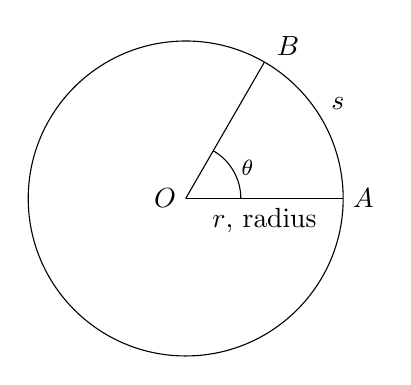
\begin{tikzpicture}[
			my angle/.style = {
				draw, angle radius=7mm, 
				angle eccentricity=1.1, 
				right, inner sep=1pt,
				font=\footnotesize
				}
			]
			\coordinate (O) at (0,0);
			\coordinate (A) at (2,0);
			\coordinate (B) at (60:2);
			\coordinate (s) at (30:2);
			\draw (O) node[anchor=east,align=center] {$O$};
			\draw (O) circle (2);
			\draw (A) node[anchor=west,align=center] {$A$};
			\draw (B) node[xshift=0.3cm, yshift=0.2cm,align=center] {$B$};
			\draw (s) node[xshift=0.2cm, yshift=0.2cm,align=center] {$s$};
			\draw (O) -- (A)node[midway, below]{$r$, radius};
			\draw (O) -- (B);
			\pic[my angle,"$\theta$"] {angle = A--O--B};
		\end{tikzpicture}
	\end{center}
\end{myleftlinebox}

\begin{myleftlinebox}
	$\pi$
	\tcblower
	$\pi$ is defined as the ratio of a circle's circumference $C$ to its diameter $d$. So $C=\pi d=2\pi r$. A right angle is $\pi/2=90$ degree.
\end{myleftlinebox}

\begin{myleftlinebox}
	trigonometric function
	\tcblower
	Given a right triangle, an angle $x$ in radian measure. For this angle $x$, define the opposite side to be the side opposite to $x$, with length $a$, define the adjacent side to be the side between $x$ and the right angle, with length $b$, and the hypotenuse side to be the side opposite to the right angle, with length $c$, then
	
	$\sin(x) = a/c$, $\cos(x)=b/c$, and $\tan(x) = a/b$; then $\csc(x)=1/\sin(x)$, $\sec(x)=1/\cos(x)$ and $\cot(x)=1/	\tan(x)$.
	\begin{center}
		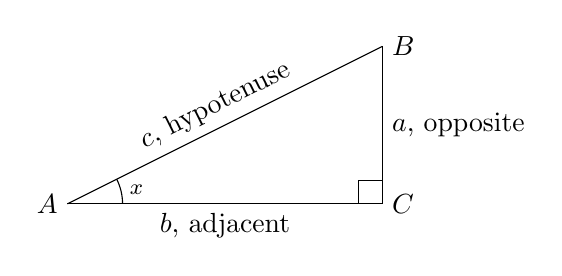
\begin{tikzpicture}[
			my angle/.style = {
				draw, angle radius=7mm, 
				angle eccentricity=1.1, 
				right, inner sep=1pt,
				font=\footnotesize
				}
			]
			\coordinate (a) at (0,0);
			\coordinate (c) at (4,0);
			\coordinate (b) at (4,2);
			\draw (a) -- (c)node[midway, below]{$b$, adjacent};
			\draw (b) -- (c)node[midway,right]{$a$, opposite};
			\draw (b) -- (a)node[midway,left, above,rotate=26.5]{$c$, hypotenuse}; % Triangle.
			\draw (a) node[anchor=east,align=center] {$A$};
			\draw (b) node[anchor=west,align=center] {$B$};
			\draw (c) node[anchor=west]{$C$};
			\draw pic[draw, angle radius=3mm] {right angle=a--c--b};
			\pic[my angle,"$x$"] {angle = c--a--b};
		\end{tikzpicture}
	\end{center}
\end{myleftlinebox}


\section{Conclusions}

\begin{myleftlinebox}
	area of circle
	\tcblower
	Using limit and squeeze theorem, we separate the area of a circle into $n$ number of annulus. Now the area of circle with radius $r$, $A$ satisfies the following:
	\[\sum_{i=0}^{n-1} \frac{r}{n}\Pare{2\pi \frac{r(i+1)}{n}}>A>\sum_{i=0}^{n-1} \frac{r}{n}\Pare{2\pi \frac{ri}{n}}\]
	\begin{center}
		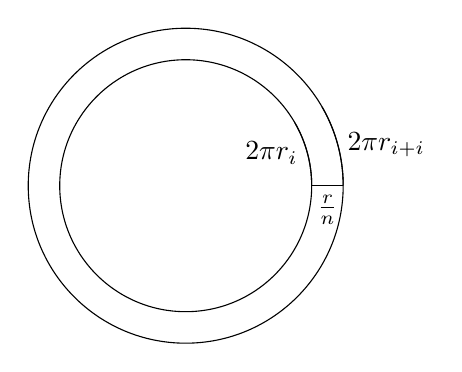
\begin{tikzpicture}[scale=0.8]
			\coordinate (O) at (0,0);
			\coordinate (A) at (2,0);
			\coordinate (B) at (2.5,0);
			\coordinate (C) at (30:2);
			\coordinate (D) at (30:2.5);
			\draw (O) circle (2);
			\draw (O) circle (2.5);
			\draw (A) arc (0:30:2)node[midway,left]{$2\pi r_i$};
			\draw (B) arc (0:30:2.5)node[midway,right]{$2\pi r_{i+i}$};
			\draw (A) -- (B)node[midway, below]{$\frac{r}{n}$};
		\end{tikzpicture}
	\end{center}
	Above inequality is reduced to 
	\[\pi r^2 \frac{n+1}{n}>A>\pi r^2 \frac{n-1}{n}\]
	Then by squeeze theorem (for series not functions), $\lim_{n\to\infty} A = A=\pi r^2$.

	Similar idea can be used to find the area of a sector. For a sector of radius $r$ and angle $\theta$, its area is $\frac{1}{2}\theta r^2$. A linear function of $\theta$.

	We can also plug in the formula for arc length $s=\theta r$ and above becomes $\frac{1}{2} \theta s$, which is quite similar to the one for triangle.
\end{myleftlinebox}


\begin{myleftlinebox}
	Pythagorean Theorem
	\tcblower
	\begin{theorem}
		In any right triangle with sides of lengths $a$ and $b$, and hypotenuse of length $c$, we have $a^2+b^2=c^2$.
	\end{theorem}
	\begin{proof}
		We can put four triangles of the same size into the following square.

		\begin{center}
			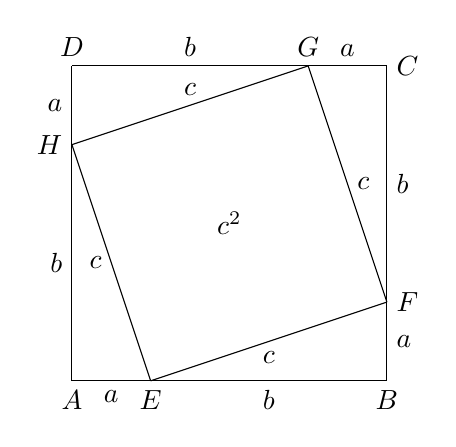
\begin{tikzpicture}
				\coordinate (A) at (-2,-2);
				\coordinate (B) at (2,-2);
				\coordinate (C) at (2,2);
				\coordinate (D) at (-2,2);
				\coordinate (O) at (0,0);
				\coordinate (E) at (-1,-2);
				\coordinate (F) at (2,-1);
				\coordinate (G) at (1,2);
				\coordinate (H) at (-2,1);
				\draw (A) node[below]{$A$};
				\draw (E) node[below]{$E$};
				\draw (B) node[below]{$B$};
				\draw (F) node[right]{$F$};
				\draw (C) node[right]{$C$};
				\draw (G) node[above]{$G$};
				\draw (D) node[above]{$D$};
				\draw (H) node[left]{$H$};
				\draw (O) node[xshift=0cm, yshift=0cm]{$c^2$};
				\draw (A) -- (E)node[midway, below]{$a$};
				\draw (E) -- (B)node[midway, below]{$b$};
				\draw (B) -- (F)node[midway, right]{$a$};
				\draw (F) -- (C)node[midway, right]{$b$};
				\draw (C) -- (G)node[midway, above]{$a$};
				\draw (G) -- (D)node[midway, above]{$b$};
				\draw (D) -- (H)node[midway, left]{$a$};
				\draw (H) -- (A)node[midway, left]{$b$};
				\draw (E) -- (F)node[midway, below]{$c$};
				\draw (F) -- (G)node[midway, right]{$c$};
				\draw (G) -- (H)node[midway, above]{$c$};
				\draw (H) -- (E)node[midway, left]{$c$};
			\end{tikzpicture}
		\end{center}
	\end{proof}
	\begin{proposition}
		$\sin^2(x)+\cos^2(x)=1$
	\end{proposition}
\end{myleftlinebox}

\begin{myleftlinebox}
	some simple relations
	\tcblower
	\begin{itemize}
		\item for any triangle with sides of length $a$, $b$, and $c$: $a+b>c$, $b+c>a$, and $c+a>b$
		\item when $x$ is close to $0$, we have $\sin(x)<x<\tan(x)$
		\begin{center}
			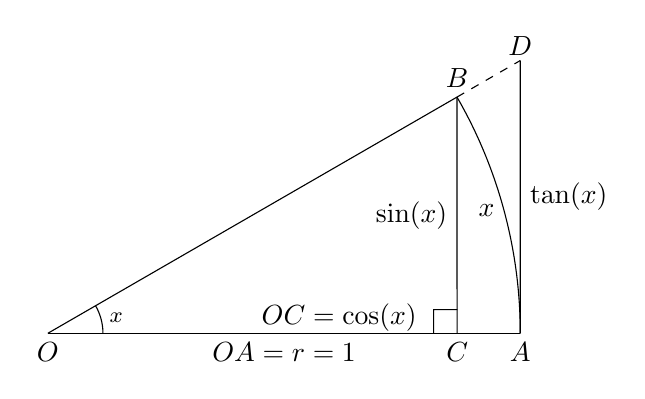
\begin{tikzpicture}[
				my angle/.style = {
					draw, angle radius=7mm, 
					angle eccentricity=1.1, 
					right, inner sep=1pt,
					font=\footnotesize
					},scale=2
				]
				\coordinate (O) at (0,0);
				\coordinate (A) at (3,0);
				\coordinate (B) at (30:3);
				\coordinate (C) at (2.6,0);
				\coordinate (D) at (3,1.7);
				\draw (A) node[below]{$A$};
				\draw (O) node[below]{$O$};
				\draw (B) node[above]{$B$};
				\draw (D) node[above]{$D$};
				\draw (O) -- (A)node[midway,below]{$OA=r=1$};
				\draw (O) -- (B);
				\draw (A) arc (0:30:3)node[midway,left]{$x$};
				\draw (B) -- (intersection of 0,0 -- 3,0 and 30:3--330:3)node[midway,left]{$\sin(x)$};
				\draw (A) -- (intersection of 3,0 -- 3,3 and 0,0--30:3)node[midway,right]{$\tan(x)$};
				\draw pic[draw, angle radius=3mm] {right angle=O--C--B};
				\draw[dashed] (B) --(intersection of 3,0--3,5 and 0,0--30:3);
				\pic[my angle,"$x$"] {angle = A--O--B};
				\draw (C) node[below]{$C$};
				\draw (O) -- (C)node[xshift=-1.5cm, yshift=0.2cm,align=center]{$OC=\cos(x)$};
			\end{tikzpicture}
		\end{center}
		\item $\tan(x)=\frac{\sin(x)}{\cos(x)}$
		\item $\sin(x+2\pi)=\sin(x)$, $\cos(x+2\pi)=\cos(x)$
		\item $\sin(-x)=-\sin(x)$, $\cos(-x)=\cos(x)$, $\tan(-x)=-\tan(x)$
		\item $\sin(x+\pi)=-\sin(x)$, $\cos(x+\pi)=-\cos(x)$
		\item $\sin(x+\pi/2)=\cos(x)$, $\cos(x+\pi/2)=-\sin(x)$
	\end{itemize}
	
\end{myleftlinebox}

\begin{myleftlinebox}
	$\sin(x+y)$ and $\cos(x+y)$
	\tcblower
	\begin{center}
		\usetikzlibrary{calc}
		\begin{tikzpicture}[
			my angle/.style = {
				draw, angle radius=7mm, 
				angle eccentricity=1.1, 
				right, inner sep=1pt,
				font=\footnotesize
				}
			]
			\coordinate (A) at (0,0);
			\coordinate (B) at (3,0);
			\coordinate (C) at (3,2);
			\coordinate (D) at (3,5);
			\draw (A) node[below]{$A$};
			\draw (B) node[below]{$B$};
			\draw (C) node[right]{$C$};
			\draw (D) node[above]{$D$};
			\draw (A) -- (B);
			\draw (A) -- (C);
			\draw (A) -- (D)node[midway,left]{$AD=1$};
			\draw (D) -- (B);
			\pic[my angle,"$x$"] {angle = B--A--C};
			\pic[my angle,"$y$"] {angle = C--A--D};
			\draw pic[draw, angle radius=3mm] {right angle=A--B--D};
			
			\coordinate (E) at ($(A)!(D)!(C)$);
			\draw (E) node[right]{$E$};
			\draw (E) -- (C);
			\draw (E) -- (D);
			\draw pic[draw, angle radius=3mm] {right angle=A--E--D};

			\coordinate (F) at ($(A)!(E)!(B)$);
			\draw (F) node[right]{$F$};
			\draw (E) -- (F);
			\draw (F) -- (B);
			\draw pic[draw, angle radius=3mm] {right angle=E--F--B};

			\coordinate (G) at ($(C)!(E)!(D)$);
			\draw (G) node[left]{$G$};
			\draw (E) -- (G);
			\draw pic[draw, angle radius=3mm] {right angle=E--G--D};
		\end{tikzpicture}
	\end{center}
	From above figure, we can write the following:
	\begin{equation*}
		\begin{split}
			&DB=\sin(x+y)=DG+GB=DG+EF\\
			&AB=\cos(x+y)=AF-AB=AF-EG\\
			&\angle CDE = \angle CAB=x\\
			&DE=AD\sin(y)=\sin(y),DG=DE\cos(x)=\sin(y)\cos(x),EG=DE\sin(x)=\sin(y)\sin(x)\\
			&AE=AD\cos(y)=\cos(y),EF=AE\sin(x)=\cos(y)\sin(x), AF=AE\cos(x)=\cos(y)\cos(x)\\
			&\sin(x+y)=\sin(x)\cos(y)+\cos(x)\sin(y)\\
			&\cos(x+y)=\cos(x)\cos(y)-\sin(x)\sin(y)
		\end{split}
	\end{equation*}
\end{myleftlinebox}

\begin{myleftlinebox}
	other formulas 
	\tcblower
	\begin{equation*}
		\begin{split}
			\tan(x+y) &= \frac{\sin(x+y)}{\cos(x+y)}=\frac{\sin(x)\cos(y)+\cos(x)\sin(y)}{\cos(x)\cos(y)-\sin(x)\sin(y)}\\
			&= \frac{\tan(x)+\tan(y)}{1-\tan(x)\tan(y)}\\
			\sin(x-y)&= \sin(x+(-y)) = \sin(x)\cos(y)-\cos(x)\sin(y)\\
			\cos(x-y)&= \cos(x+(-y)) = \cos(x)\cos(y)+\sin(x)\sin(y)\\
			\tan(x-y)&= \tan(x+(-y)) =  \frac{\tan(x)-\tan(y)}{1+\tan(x)\tan(y)}\\
			\sin(2x) &= \sin(x+x) = 2\sin(x)\cos(x)=\frac{2\sin(x)\cos(x)}{\sin^2(x)+\cos^2(x)} = \frac{2\tan(x)}{1+\tan^2(x)}\\
			\cos(2x) &= \cos(x+x) = \cos^2(x)-\sin^2(x)=\frac{\cos^2(x)-\sin^2(x)}{\sin^2(x)+\cos^2(x)} = \frac{1-\tan^2(x)}{1+\tan^2(x)}\\
			\tan(2x) &= \tan(x+x) = \frac{2\tan(x)}{1-\tan^2(x)}
		\end{split}
	\end{equation*}
\end{myleftlinebox}

\begin{myleftlinebox}
	half-angle formulas 
	\tcblower
	use the identity:
	\begin{equation*}
		\begin{split}
			\cos(2x)&=2\cos^2(x)-1=1-2\sin^2(x)\\
			\cos(x) &=2\cos^2(x/2)-1=1-2\sin^2(x/2)
		\end{split}
	\end{equation*}
	then solve this quadratic equation we have
	\begin{equation*}
		\begin{split}
			\sin(x/2) &= \sqrt{\frac{\cos(x)+1}{2}} \text{ or } -\sqrt{\frac{\cos(x)+1}{2}}\\
			\cos(x/2) &= \sqrt{\frac{1-\cos(x)}{2}} \text{ or } -\sqrt{\frac{1-\cos(x)}{2}}
		\end{split}
	\end{equation*}
	where the sign can be determined using the quadrant of the half-angle.  
\end{myleftlinebox}

\begin{myleftlinebox}
	Law of sines
	\tcblower
	\begin{theorem}
		For any triangle $\triangle ABC$ with sides of length $a$, $b$, $c$, we have the following:
		\[\frac{a}{\sin(\angle A)}=\frac{c}{\sin(\angle C)}=\frac{b}{\sin(\angle B)}\]
		\begin{center}
			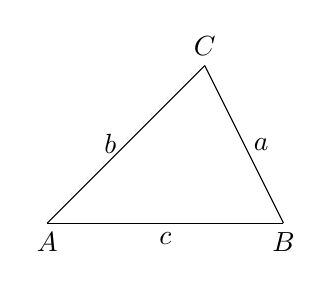
\begin{tikzpicture}
				\coordinate (A) at (0,0);
				\coordinate (B) at (3,0);
				\coordinate (C) at (2,2);
				\draw (A) node[below]{$A$};
				\draw (B) node[below]{$B$};
				\draw (C) node[above]{$C$};
				\draw (A) -- (B)node[midway,below]{$c$};
				\draw (A) -- (C)node[midway,left]{$b$};
				\draw (C) -- (B)node[midway,right]{$a$};
			\end{tikzpicture}
		\end{center}
	\end{theorem}
	The proof uses the fact that the area of this triangle $S=\frac{1}{2}c\cdot b\sin\angle A=\frac{1}{2}c\cdot a\sin\angle B$
\end{myleftlinebox}

\begin{myleftlinebox}
	Law of cosines
	\tcblower
	\begin{theorem}
		For any triangle $\triangle ABC$ with sides of length $a$, $b$, $c$, we have the following:
		\begin{align*}
			c^2 &= a^2+b^2 -2ab\cos\angle C\\
			a^2 &= b^2+c^2 -2bc\cos\angle A\\
			b^2 &= c^2+a^2 -2ca\cos\angle B
		\end{align*}
	\end{theorem}
	\begin{proof}
		Notice that $c=a\cos\angle B+b\cos\angle A$, we multiply this by $c$ and obtain
		\[c^2=ac\cos\angle B+bc\cos\angle A\]
		Do this for all three sides and we have
		\begin{align*}
			a^2 &= ac\cos\angle B+ab\cos\angle C\\
			b^2 &= bc\cos\angle A+ba\cos\angle C\\
			c^2 &= ca\cos\angle B+cb\cos\angle A
		\end{align*}
		And the rest part of the proof is obvious.
	\end{proof}
\end{myleftlinebox}

\section{Extensions}

\begin{myleftlinebox}
	inverse trigonometric functions, not the reciprocal trigonometric functions
	\tcblower
	With $y=\sin(x)$, where $x\in \bR$, we define $x=\arcsin(y)$ where $y\in[-1,1]$ and range $x\in [-\frac{\pi}{2},\frac{\pi}{2}]$. Similarly we can define the following:
	\begin{itemize}
		\item $y=\arcsin(x)$ where $x\in[-1,1]$ and $y\in [-\frac{\pi}{2},\frac{\pi}{2}]$
		\item $y=\arccos(x)$ where $x\in[-1,1]$ and $y\in [0,\pi]$
		\item $y=\arctan(x)$ where $x\in\bR$ and $y\in [-\frac{\pi}{2},\frac{\pi}{2}]$
	\end{itemize}
\end{myleftlinebox}

\begin{myleftlinebox}
	composition of inverse trigonometric functions
	\tcblower
	We have the following result:
	\begin{center}
		\begin{tabular}{lll}
			$\sin(\arcsin(x))=x$ & $\cos(\arcsin(x))=\sqrt{1-x^2}$ & $\sin(\arccos(x))=\sqrt{1-x^2}$\\
			$\sin(\arccos(x))=\sqrt{1-x^2}$ & $\cos(\arccos(x))=x$ & $\tan(\arccos(x))=\frac{\sqrt{1-x^2}}{x}$\\
			$\sin(\arctan(x))=\frac{x}{\sqrt{1+x^2}}$ & $\cos(\arctan(x))=\frac{1}{\sqrt{1+x^2}}$ & $\tan(\arctan(x))=x$
		\end{tabular}
	\end{center}
\end{myleftlinebox}

\begin{myleftlinebox}
	relation between inverse trigonometric functions
	\tcblower
	We have the following result:
	\begin{align*}
		\arcsin(-x) &= -\arcsin(x)\\
		\arccos(-x) &= \pi-\arccos(x)\\
		\arctan(-x) &= -\arctan(x)\\
		\arccos(x) &= \frac{\pi}{2}-\arcsin(x)\\
		\arctan(\frac{1}{x}) &= \frac{\pi}{2}- \arctan(x), x>0\\
		\arctan(\frac{1}{x}) &= -\frac{\pi}{2}- \arctan(x), x<0
	\end{align*}
\end{myleftlinebox}

\begin{myleftlinebox}
	hyperbolic functions
	\tcblower
	Using exponential function $e^x$ we define:
	\begin{align*}
		\sinh(x) &= \frac{e^x-e^{-x}}{2} = \frac{e^{2x}-1}{2e^x} = \frac{1-e^{-2x}}{2e^{-x}}\\
		\cosh(x) &= \frac{e^x+e^{-x}}{2} = \frac{e^{2x}+1}{2e^x} = \frac{1+e^{-2x}}{2e^{-x}}\\ 
		\tanh(x) &= \frac{\sinh(x)}{\cosh(x)} = \frac{e^x-e^{-x}}{e^x+e^{-x}} = \frac{e^{2x}-1}{e^{2x}+1}
	\end{align*}
\end{myleftlinebox}

\begin{myleftlinebox}
	relation between hyperbolic functions
	\tcblower
	Using exponential function $e^x$ we define:
	\begin{align*}
		\sinh(-x) &= -\sinh(x)\\
		\cosh(-x) &= \cosh(x)\\
		\cosh^2(x) -\sinh^2(x) &= 1\\
		\cosh(x)+\sinh(x)&=e^x\\
		\cosh(x)-\sinh(x)&=e^{-x}\\
		\sinh(x+y) &=\sinh(x)\cosh(y)+\cosh(x)\sinh(y)\\
		\cosh(x+y) &=\cosh(x)\cosh(y)+\sinh(x)\sinh(y)\\
		\arcsinh(x)&=\ln(\sqrt{x+\sqrt{x^2+1}})\\
		\arccosh(x)&=\ln(\sqrt{x+\sqrt{x^2-1}})\\
	\end{align*}
\end{myleftlinebox}

\section{Exercises}

\begin{myleftlinebox}
	show that $\frac{\sin(x)}{x}\to 1$ as $x\to 0$.
	\tcblower
	\vspace{2em}
\end{myleftlinebox}

\begin{myleftlinebox}
	show that $\frac{1-\cos(x)}{0.5x^2}\to 1$ as $x\to 0$.
	\tcblower
	\vspace{2em}
\end{myleftlinebox}

\begin{myleftlinebox}
	show that $\frac{\tan(x)}{x}\to 1$ as $x\to 0$.
	\tcblower
	\vspace{2em}
\end{myleftlinebox}

\end{document}
